\section{Localization within a proof}\label{sec:loc}

\begin{table}[t]
\caption{Exact first-rejection localization on eligible failed proofs (\%, equal attempt weights). N/G: attempts/tasks (exercise groups on ProofNet). Uniform is the average of $1/L$; First step always predicts $\hat t=1$; Prior is a positional localizer fitted on first-rejection positions of calibration failures (Appendix~\ref{app:temp}). Temperature-1.0 rows use rules and priors frozen from the 0.6 analysis.}
\label{tab:main}
\begin{center}
\small
\setlength{\tabcolsep}{4pt}
\begin{tabular}{llcrrrrrr}
\toprule
Dataset & Model & Temp. & N/G & Jump & Uniform & First step & Prior & Surprisal\\
\midrule
miniF2F & DeepSeek & 0.6 & 528/122 & 24.4 & 9.7 & 7.6 & 18.2 & 17.6\\
miniF2F & Goedel & 0.6 & 448/122 & 25.4 & 8.7 & 6.5 & 14.7 & 13.2\\
miniF2F & Kimina & 0.6 & 324/94 & 17.3 & 8.7 & 9.9 & 11.7 & 12.0\\
ProofNet & DeepSeek & 0.6 & 456/167 & 20.4 & 13.3 & 21.7 & 19.3 & 22.6\\
ProofNet & Goedel & 0.6 & 262/134 & 29.4 & 14.2 & 31.7 & 25.6 & 22.5\\
\midrule
miniF2F & DeepSeek & 1.0 & 544/140 & 20.4 & 10.3 & 6.4 & 20.4 & 16.0\\
miniF2F & Goedel & 1.0 & 456/124 & 20.2 & 9.1 & 6.6 & 16.2 & 14.0\\
miniF2F & Kimina & 1.0 & 498/122 & 19.1 & 10.7 & 9.6 & 13.5 & 12.1\\
\bottomrule
\end{tabular}
\end{center}
\end{table}

\paragraph{The largest increment points to the first rejection (P2).} At temperature 0.6 the jump argmax matches the first rejection in 17.3--25.4\% of eligible miniF2F failures and 20.4--29.4\% of ProofNet failures, 1.5--2.9 times the uniform reference (Table~\ref{tab:main}). It exceeds the surprisal argmax in every miniF2F cell; on ProofNet the prespecified contrasts, jump minus surprisal, are $-2.58$\,pp $[-8.58, 3.29]$ for DeepSeek and $+5.19$\,pp $[-2.15, 12.53]$ for Goedel (97.5\% intervals). With all rules frozen, the result replicates at temperature 1.0 for all three provers: 19.1--20.4\% against 9.1--10.7\% uniform (Holm-adjusted one-sided $p\le6.1\times10^{-4}$), 4.4--7.0 points above surprisal. Within one step, the jump exceeds surprisal clearly only for Kimina (Appendix~\ref{app:temp}).

\paragraph{On ProofNet the advantage is positional.} Failures there concentrate at the first step: on the learned-comparison population, 99/452 (DeepSeek) and 83/259 (Goedel) attempts fail at step 1, and none at the last step. The first-step rule reaches 21.7\% and 31.7\%, against 20.4\% and 29.4\% for the jump argmax, and a fitted positional prior differs from the jump by $+1.1$ and $+3.8$\,pp, with intervals containing zero (Table~\ref{tab:main}, Appendix~\ref{app:temp}). Removing step~1 from the candidates costs the jump 1.8\,pp for DeepSeek and 10.7\,pp for Goedel. Within one step, the jump argmax is the strongest single signal (43.2\% and 48.2\%; Table~\ref{tab:learned}).

\paragraph{On miniF2F the jump exceeds position.} The first-step rule reaches 6.4--9.9\%, and the jump exceeds it by 7--19\,pp. Against the fitted prior, the jump gains $+10.7$\,pp $[4.8, 17.1]$ for Goedel and $+6.3$\,pp $[0.4, 12.5]$ for DeepSeek at temperature 0.6, and $+5.6$\,pp $[-2.1, 13.1]$ for Kimina. With equal task weights the Goedel gain persists ($+9.9$\,pp), the Kimina gain becomes clear ($+8.2$\,pp $[1.8, 14.8]$) and the DeepSeek gain vanishes ($+0.2$\,pp). At temperature 1.0 the gains are $0.0$ to $+5.6$\,pp, with lower bounds at or below zero (Appendix~\ref{app:temp}).

\begin{table}[t]
\caption{Single-signal and learned localizers on the learned-comparison ProofNet population (\%, equal exercise-group weights). $\pm1$: $|\hat t-t^*|\le1$. M0/M1 predictions are out of fold (Section~\ref{sec:learned}).}
\label{tab:learned}
\begin{center}
\begin{tabular}{lrrrr}
\toprule
& \multicolumn{2}{c}{DeepSeek (452/166)} & \multicolumn{2}{c}{Goedel (259/133)}\\
\cmidrule(lr){2-3}\cmidrule(lr){4-5}
Localizer & Exact & $\pm1$ & Exact & $\pm1$\\
\midrule
Uniform & 12.55 & 32.00 & 13.15 & 32.19\\
First step & 19.81 & 35.31 & 28.66 & 40.78\\
Argmax surprisal & 21.40 & 36.81 & 21.27 & 43.75\\
Argmax jump & 18.50 & 43.21 & 26.57 & 48.15\\
M0: position, span, tactic, surprisal & 40.85 & 52.05 & 57.82 & 66.30\\
M1: M0 features plus jump & 43.51 & 54.28 & 57.13 & 65.49\\
\bottomrule
\end{tabular}
\end{center}
\end{table}

\begin{table}[t]
\caption{Prefix-restricted localization: argmax of $w_t$ over $t\le t^*$, failed attempts with $t^*\ge2$ (\%). Uniform is the average of $1/t^*$. Control: for a cutoff $k=t^*$, the rate at which step $k$ is the maximum of the prefix $1,\dots,k$ in failed proofs whose first rejection comes after $k$ (Appendix~\ref{app:temp}); Supported: hit rate on attempts whose cutoff has such proofs. Differences in percentage points with 95\% task/group bootstrap intervals.}
\label{tab:prefix}
\begin{center}
\scriptsize
\setlength{\tabcolsep}{3pt}
\begin{tabular}{llrrcrrc}
\toprule
Dataset & Model & Prefix hit & Uniform & $\Delta$ vs uniform & Supported & Control & $\Delta$ vs control\\
\midrule
miniF2F & DeepSeek & 38.52 & 16.97 & $+21.56$ [15.20, 27.99] & 38.60 & 25.89 & $+12.71$ [6.83, 18.63]\\
miniF2F & Goedel & 38.19 & 16.51 & $+21.67$ [15.32, 27.98] & 38.28 & 23.92 & $+14.36$ [8.07, 20.91]\\
miniF2F & Kimina & 35.27 & 16.71 & $+18.57$ [11.57, 26.12] & 35.52 & 21.40 & $+14.12$ [7.10, 21.82]\\
ProofNet & DeepSeek & 42.86 & 24.76 & $+18.10$ [12.69, 23.48] & 42.98 & 34.80 & $+8.18$ [3.09, 13.28]\\
ProofNet & Goedel & 41.34 & 24.40 & $+16.94$ [10.07, 23.78] & 41.57 & 24.93 & $+16.65$ [9.92, 23.02]\\
\bottomrule
\end{tabular}
\end{center}
\end{table}

\paragraph{Within a proof, the rejected step stands out beyond position.} Restricting candidates to steps $1,\dots,t^*$ removes text generated after the rejection. The rejected step then carries the largest increment in 35.3--42.9\% of proofs, against 16.5--24.8\% for a uniform choice (Table~\ref{tab:prefix}). A monotone trend of $w_t$ in position would also favor the last step of a prefix, so we apply the same rule at the same cutoff $k$ to failed proofs whose first rejection comes after $k$: their step $k$ was accepted, and it is the prefix maximum in 21.4--34.8\% of them. The rejected step exceeds this control by 8.2--16.7\,pp, with intervals above zero in all five cells. The control lies 0.5--10.0\,pp above the uniform reference, so part of the gain over uniform is positional and the rest is specific to failure.

\paragraph{Read-out choices.} The prefix effect holds for whitened scores at the quarter, middle and three-quarter layers, at shrinkage 0.01 and 0.5, and with a transform fitted on a second calibration fold: the contrast with the control ranges from $+5.6$ to $+22.2$\,pp with every interval above zero, and is largest at the quarter layer on miniF2F (Appendix~\ref{app:sensitivity}). Whitening matters on miniF2F: with raw increment norms the contrast falls to $+3.2$ to $+7.3$\,pp and turns negative for Goedel ($-1.4$\,pp), and full-proof exact localization drops to 5.1--13.9\%. On ProofNet, whose transform is fitted on miniF2F, raw norms localize as well as or better than whitened ones (26.3\% and 30.2\%). Refitting the transform on the second fold changes exact localization by $-3.8$ to $+0.7$\,pp but moves the argmax in 15--38\% of attempts: the rate is stable, the argmax of an individual proof is not.

\section{Why the maximum misses: coupling and clustering}\label{sec:why}

Theorem~\ref{thm:loc} attributes perfect localization to coupling (the first rejection is the first exceedance of a fixed tolerance) and extremal independence (large steps do not cluster). For thresholds $u_q$, the $q$-quantiles of increments on verified calibration proofs, let $M=\max_tw_t$, $F=\min\{t:w_t>u_q\}$ and $T$ the earliest argmax. We measure (a) trace-level coupling, $\PP(M>u_q)$ in failed versus verified proofs of the same tasks; (b) clustering, $\PP(T=F\mid M>u_q)$ in failed proofs; and (c) step-level coupling, $\PP(F=t^*\mid M>u_q)$ in failed proofs.

\begin{table}[t]
\caption{Threshold diagnostics at $q=0.95$ (\%, 95\% task/group bootstrap intervals); (b) and (c) are conditional on $M>u$ in failed proofs. Verified proofs come from the same tasks or groups as the failed ones; ProofNet verified cells are descriptive (35 and 40 attempts). All quantiles in Table~\ref{tab:allq}.}
\label{tab:threshold}
\begin{center}
\small
\begin{tabular}{llcccc}
\toprule
& & \multicolumn{2}{c}{(a) $\PP(M>u)$} & (b) $T=F$ & (c) $F=t^*$\\
\cmidrule(lr){3-4}\cmidrule(lr){5-5}\cmidrule(lr){6-6}
Dataset & Model & Failed & Verified & Failed & Failed\\
\midrule
miniF2F & DeepSeek & 44.1 [36.2, 52.4] & 25.0 [16.1, 35.5] & 48.9 [39.9, 57.6] & 15.0 [7.1, 24.0]\\
miniF2F & Goedel & 50.5 [42.1, 58.4] & 29.0 [19.4, 40.2] & 37.2 [28.6, 46.8] & 17.7 [9.4, 26.9]\\
miniF2F & Kimina & 57.7 [47.9, 67.4] & 35.5 [24.0, 48.0] & 38.0 [29.0, 47.6] & 19.8 [11.7, 28.8]\\
ProofNet & DeepSeek & 84.7 [79.7, 89.2] & 62.9 & 25.9 [20.9, 31.3] & 22.5 [17.1, 28.0]\\
ProofNet & Goedel & 87.8 [83.0, 92.1] & 75.0 & 23.5 [17.1, 30.3] & 26.1 [18.2, 34.3]\\
\bottomrule
\end{tabular}
\end{center}
\end{table}

\begin{figure}[t]
\begin{center}
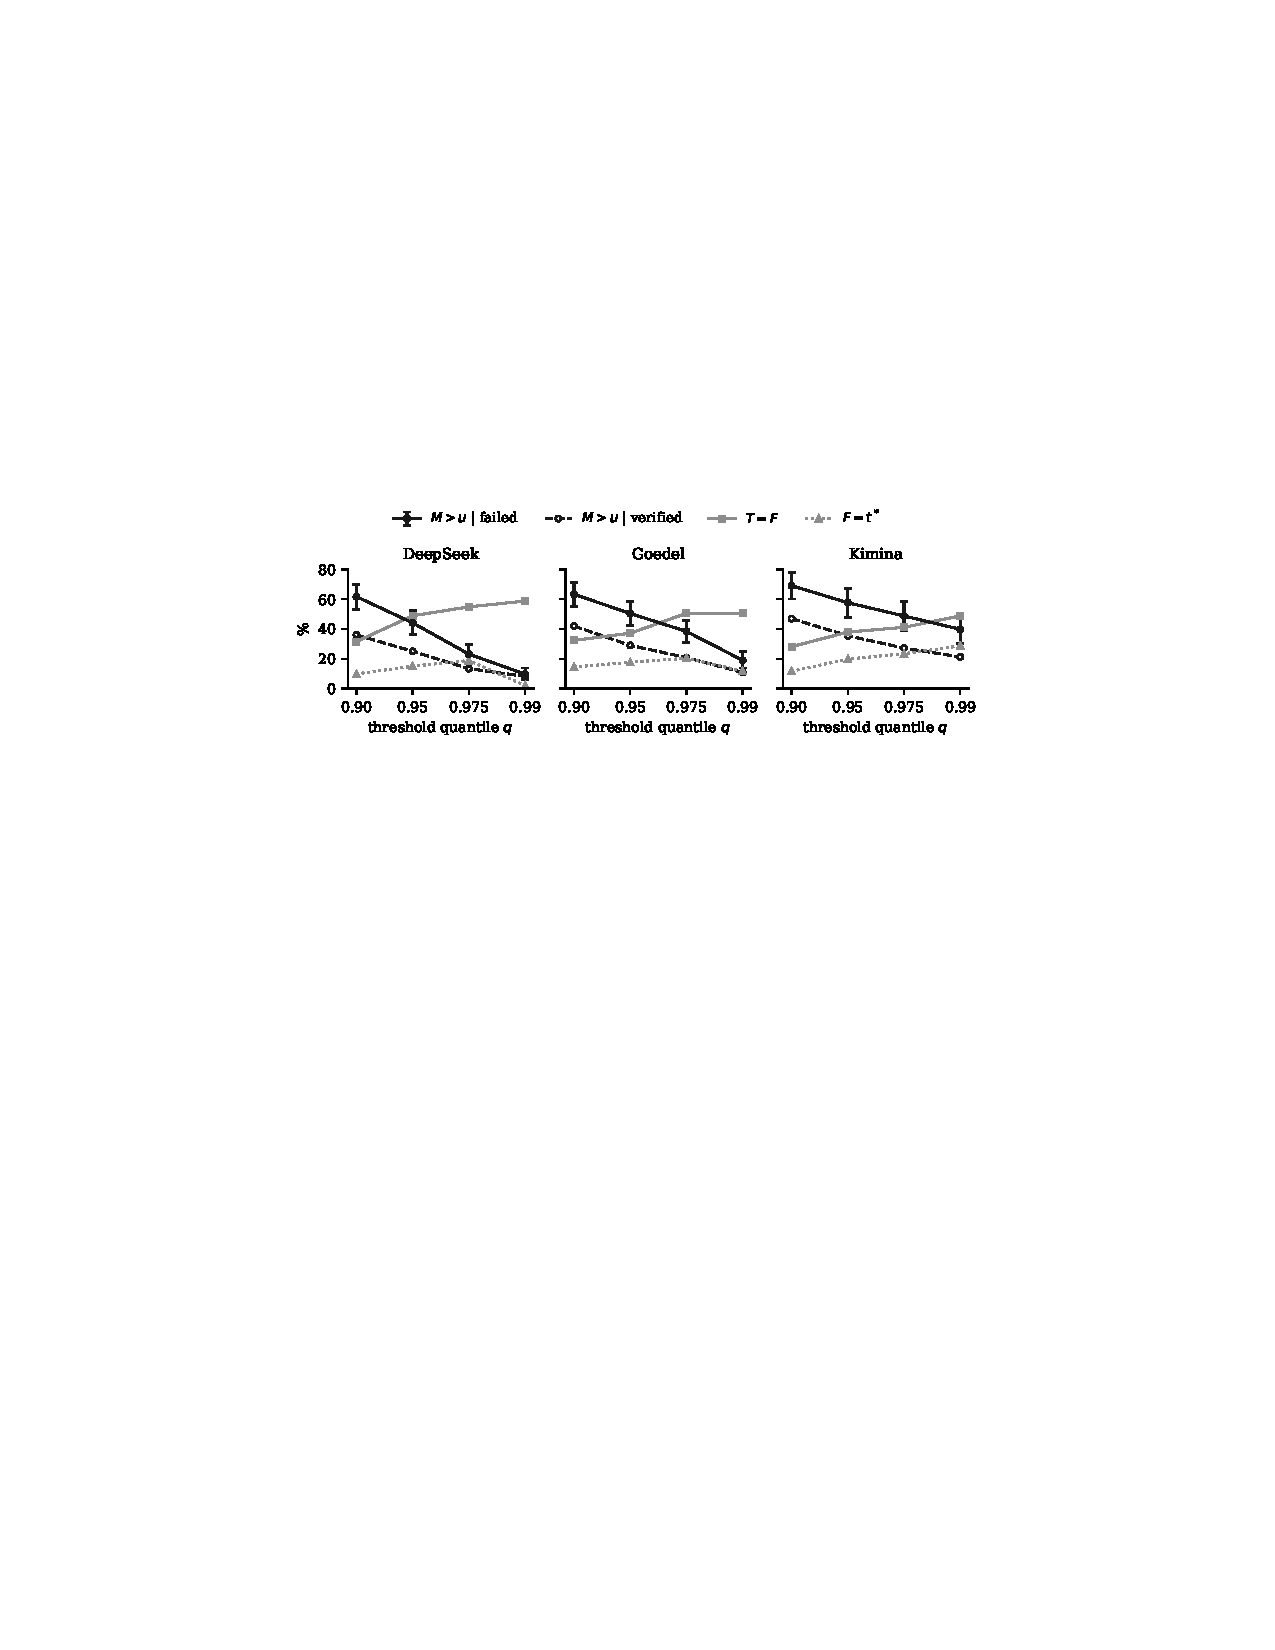
\includegraphics[width=0.95\linewidth]{fig_threshold.pdf}
\end{center}
\caption{Threshold diagnostics on miniF2F across quantiles $q$ of verified calibration increments. Failed proofs exceed the threshold more often than verified proofs of the same tasks (black), but the first exceedance rarely falls on the rejected step (grey dotted), and the maximum coincides with the first exceedance in only 28--59\% of cases (grey solid). Error bars: 95\% task-bootstrap intervals.}
\label{fig:threshold}
\end{figure}

\paragraph{Exceedance is more frequent in failed proofs but does not identify failure.} At $q=0.95$ on miniF2F, 44--58\% of failed proofs exceed the threshold against 25--35\% of verified proofs of the same tasks (Table~\ref{tab:threshold}), and the gap persists at every quantile (Figure~\ref{fig:threshold}). At no threshold does exceedance separate the two outcomes: failed proofs without an exceedance and verified proofs with one are both common.

\paragraph{Step-level coupling is the main loss; clustering is the second.} When a failed proof exceeds the threshold, its first exceedance is the rejected step in 15--20\% of miniF2F cases and 23--26\% on ProofNet at $q=0.95$, and never more than a third at any quantile. Clustering compounds this: the maximum coincides with the first exceedance in 37--49\% of miniF2F cases at $q=0.95$ and 49--59\% at $q=0.99$, so a later and larger step often follows the first one. Under the theorem's conditions both quantities would tend to one.

\paragraph{The absolute scale shifts across benchmarks.} With the whitening transform and thresholds calibrated on miniF2F, 85--88\% of failed and 63--75\% of verified ProofNet proofs exceed the $q=0.95$ threshold. The same fixed transform places ProofNet increments far higher, so a tolerance calibrated on one benchmark does not carry over to another. Together with Section~\ref{sec:loc}, these diagnostics locate the departure from Hypothesis~\ref{hyp:coupling} in its absolute tolerance: the rejected step is extreme \emph{relative to its own proof}, not beyond a common level.

\section{Online alarms}\label{sec:online}

A relative marker is hard to use online, where each step is judged before the rest of the proof exists. We fit a discrete hazard model on ProofNet: for failed attempts the steps $1,\dots,t^*$ enter with target $\1\{t=t^*\}$, and verified attempts of the same groups enter with all steps as survivors. The baseline H0 uses only past and present features (step index, $\log t$, span length, tactic category, surprisal and its running statistics); H1 adds $\log(1+w_t)$, the running maximum of $w$ and the ratio of $w_t$ to that maximum. Both use the nested group cross-validation of Section~\ref{sec:learned}. An alarm fires at the first step whose hazard exceeds a threshold set on inner out-of-fold verified attempts for a target false-alarm rate.

Online exact localization is 8--21\%, and the jump features change it by $-0.45$\,pp in the primary cell ($[-2.51, 1.86]$) and by $-4.47$ to $+1.63$\,pp elsewhere (Table~\ref{tab:online}, Appendix~\ref{app:temp}). Realized false-alarm rates depart from their targets (15.6\% at a 10\% target for DeepSeek): an alarm level calibrated on held-out verified proofs transfers imperfectly, as the threshold diagnostics of Section~\ref{sec:why} predict. Online, the jump adds nothing measurable to position and surprisal.


\section{Added value beyond cheap step features}\label{sec:learned}

\paragraph{Design.} We compare two independently fitted ridge-regularized conditional-logit localizers \citep{mcfadden1974}. For attempt $i$, each assigns a distribution over candidate steps,
\begin{equation}\label{eq:clogit}
p_{it}^{(m)}=\frac{\exp(r_{it}^{(m)})}{\sum_{s=1}^{L_i}\exp(r_{is}^{(m)})},\qquad r_{it}^{(0)}=\theta_0^\top\phi(b_{it}),\qquad r_{it}^{(1)}=\theta_1^\top\phi(b_{it})+\beta u_{it}.
\end{equation}
Baseline features are step index $t$, relative position $t/L_i$, first/last-step indicators, $\log(1+n_{it})$ for token-span length, AST tactic category and mean surprisal, with cubic B-splines for the four numeric features; $u_{it}$ is standardized $\log(1+w_{it})$ and $\beta$ is unconstrained in sign. The loss is the negative log-probability of $t_i^*$ with equal total weight per exercise group, under five outer and three inner group folds \citep{varma2006}; all preprocessing and the ridge parameter are fitted within training splits, and paired intervals resample whole groups 20,000 times on the saved out-of-fold predictions (Appendix~\ref{app:incremental}).


\paragraph{Results.} The learned localizer M0 is far stronger than any single signal (40.9\% and 57.8\% exact; Table~\ref{tab:learned}). For DeepSeek, the primary cell, adding the jump raises exact localization to 43.5\%, a gain of $+2.66$\,pp ($[0.45, 5.17]$; 97.5\% family interval $[0.25, 5.57]$), with 14 attempts corrected and 6 lost, concentrated in short proofs and first-step failures (Table~\ref{tab:strata}). For Goedel, exact localization changes by $-0.69$\,pp ($[-3.13, 1.57]$). With 133 groups this cell detects effects of about 3.4\,pp at 80\% power, so the change in exact localization is inconclusive; its out-of-fold NLL is worse by 0.056 nats ($[0.023, 0.092]$; Table~\ref{tab:incremental}, Appendix~\ref{app:incremental}). With M0 and M1 refitted on miniF2F at temperature 0.6 and frozen, the DeepSeek gain does not transfer to temperature-1.0 samples (Holm-adjusted one-sided $p=0.48$). The standardized jump coefficient is positive in every outer fold for both provers (0.11--0.42): conditional on position, span, tactic and surprisal, larger increments mark the first rejection.

\paragraph{Agreement with surprisal.} When the jump and surprisal maxima fall on the same or adjacent steps (23--45\% of eligible failures), the region of at most two steps contains the first rejection in 45--60\% of them, 1.4--2.0 times as often as a random window of the same size (Appendix~\ref{app:agreement}). Against single signals given the same number of candidates on proofs of the same length, all ten differences are positive (+2 to +17 points), and three exclude zero after Bonferroni correction over 40 contrasts. As a detector of failed proofs, agreement adds nothing to length. When two signals of different nature point to neighboring steps, the first failure lies there; this within-proof property carries no cross-proof information, as Section~\ref{sec:why} predicts.

\section{Other predictions of the framework}\label{sec:other}

\paragraph{Success versus length (P5).} Following Proposition~\ref{prop:length}, we test Qwen2.5-7B-Instruct \citep{qwen2024} on synthetic modus-ponens chains with distractors \citep{saparov2023}, with assigned lengths $L=3,\dots,12$, 1,000 calibration and 500 held-out tasks per temperature, and a symbolic checker. A one-parameter model $p_c(L)=\exp(-cL)$ fitted on calibration outcomes lowers held-out Brier score from 0.1398 to 0.1269 at temperature 1.0 ($c=0.268$), an improvement of 9.2\% (97.5\% interval $[0.0024, 0.0242]$ in absolute terms), and by 0.0065 ($[-0.0040, 0.0178]$) at 0.6. Success decays with length, but the exponential form is not specific: linear, Weibull, nonparametric and two further parametric models reach 0.1266--0.1274 at temperature 1.0, and the nonparametric model is best at 0.6 (0.1388 against 0.1424). The hazard of the first locally invalid inference also changes with step index (likelihood-ratio tests against a constant hazard, $p\le10^{-4}$; Appendix~\ref{app:dynamics}). Length is predictive, but the constant-hazard mechanism behind Proposition~\ref{prop:length} is not supported.

\paragraph{Tail behavior (P1, P3, P4).} No Pareto law appears at the first rejection (P3), consistent with the absence of a common threshold in Section~\ref{sec:why}. For P1, refuted-minus-verified moment-estimator contrasts have 95\% intervals $[-1.333, 0.754]$, $[-0.239, 0.141]$ and $[-0.995, 0.353]$ for DeepSeek, Goedel and Kimina (Appendix~\ref{app:tails}). The peak-to-neighbor ratio of the maximum shows no outcome effect after length and task adjustment. For P4, in five paired modular-addition trainings \citep{nanda2023}, signed tail estimates are nonpositive before and after the generalization transition and for shuffled-label controls. The supported content of the framework is its localization structure.

\section{Related work}

\paragraph{Extreme values and recurrences.} Tail processes describe dependence around large observations \citep{basrak2009,kulik2020}, and the extremal index links clustering to limits of maxima \citep{leadbetter1983}. Kesten--Goldie theory \citep{kesten1973,goldie1991,buraczewski2016} yields heavy tails of SGD iterates \citep{gurbuzbalaban2021,hodgkinson2021}; heavy tails also appear in gradient noise \citep{simsekli2019} and weight spectra \citep{martin2021}.

\paragraph{Error signals and formal reasoning.} Hidden-state probes detect falsehoods and hallucinations \citep{azaria2023,orgad2025}, semantic entropy detects confabulation \citep{farquhar2024}, and process supervision assesses individual reasoning steps \citep{lightman2024}. The provers we study generate verifiable Lean proofs \citep{ren2025,lin2025,wang2025}; compositionality studies model failure as compounding per-step error \citep{dziri2023,saparov2023}, and work on modular addition \citep{nanda2023} and heuristic arithmetic \citep{nikankin2025} motivates the algorithm/heuristic contrast behind the tail regimes.

\section{Discussion and conclusion}\label{sec:discussion}

One of the five predictions fixed in advance is confirmed: the largest residual change marks the first rejected step (P2). Within a proof the effect exceeds a positional control in every cell and survives changes of layer, shrinkage and calibration fold; across the full proof it exceeds the first-step rule on miniF2F and a fitted positional prior in some miniF2F cells, but not position on ProofNet. Success decays with length (P5), but not through the constant hazard the framework proposes. The three tail predictions (P1, P3, P4) fail.

The framework explains why the maximum misses. Its idealized limit requires that rejection coincide with crossing a fixed tolerance and that large steps not cluster. The data break the first condition most: failed proofs exceed a fixed level more often than verified ones, but the first exceedance rarely lands on the rejected step, and the scale shifts between benchmarks. Clustering is the second loss. What survives is extremality within a trace.

Appendix~\ref{app:protocol} specifies a confirmatory test of these results on new tasks.

\section*{Reproducibility statement}
Appendix~\ref{app:proofs} gives the proofs; Appendices~\ref{app:readout}--\ref{app:dynamics} and \ref{app:sensitivity} give read-out, segmentation, frozen revisions, the group-weighted objective, feature preprocessing, nested cross-validation, positional references, the prefix control, length models, read-out sensitivity and uncertainty procedures. The experimental archive fixes code and data by SHA256 before localizer fitting and records group splits, preprocessing parameters, coefficients, per-step out-of-fold predictions, per-group contrasts, bootstrap replicates and per-attempt exclusions. Reproduction additionally requires the prompts and the executable model and Lean environments. Appendix~\ref{app:protocol} gives the confirmatory protocol.

\section*{AI use statement}
AI tools assisted with manuscript editing and with checks of consistency between manuscript claims and reported experimental results.
